\section{Hardware Implementation}
With the hardware components being chosen, it is necessary to assemble them, ensure that they are compatible for communication with the microcontroller, and that they receive the appropriate electrical power. Other implementation considerations also have to be considered. e.g , the voltage divider for the power monitor.
\subsection{Microcontroller peripherals}
Before choosing which pins on the Arduino Mega to connect the various hardware to, the peripherals\footnote{Hardware modules, such as timers, UARTs, etc.} in the microcontroller needs to be evaluated (each peripheral is only available on certain pins). First, the timers are considered. The microcontroller has 6 hardware timers, Timer 0 to Timer 5.

Timer 0 is reserved by the Arduino for it's internal time keeping functions, and not to be touched \cite{ArduinoPWM}. This leaves 5 timers, that can be used freely.

It would be advantageous to utilize the input capture\footnote{An input capture timer samples a free running counter, whenever triggered by  an external event} functionality of the timers to read the hall sensors, since it will provide a hardware generated timestamp, and be independent of software latency. After examining the Arduino Mega pinout, \appref{megaPinout}, it is seen that only Timer 4 and 5 have their input capture pins available on the board (ICP4 and ICP5). These are therefore chosen for the two hall sensors.
   
The real-time operating system needs a timer, for running its scheduler. Timer 1 is chosen for this, for no other reason than it being the default setting.

This leaves Timer 2 and 3. According to \cite{Atmega}, Timer 2 is an 8 bit timer, and Timer 3 is 16 bit. 

Timer 3 is chosen for the PWM signal sent to the servo. This, because the higher resolution makes it easier to generate the short duty cycles required by the servo (\si{500\ \mu s} to \si{2500\ \mu s} on-time, in a \si{30\ ms} period, see \subsecref{Servo})

The last timer is chosen for the PWM signal to the DC-motor.

As the timers have now been designated, the next step is to assign the various serial ports. This is done as shown on \figref{MegaSetup}. Considerations about the powering of the hardware modules is seen in \secref{sec:elecConsiderations}.	


\begin{figure}[H]
	\centering
	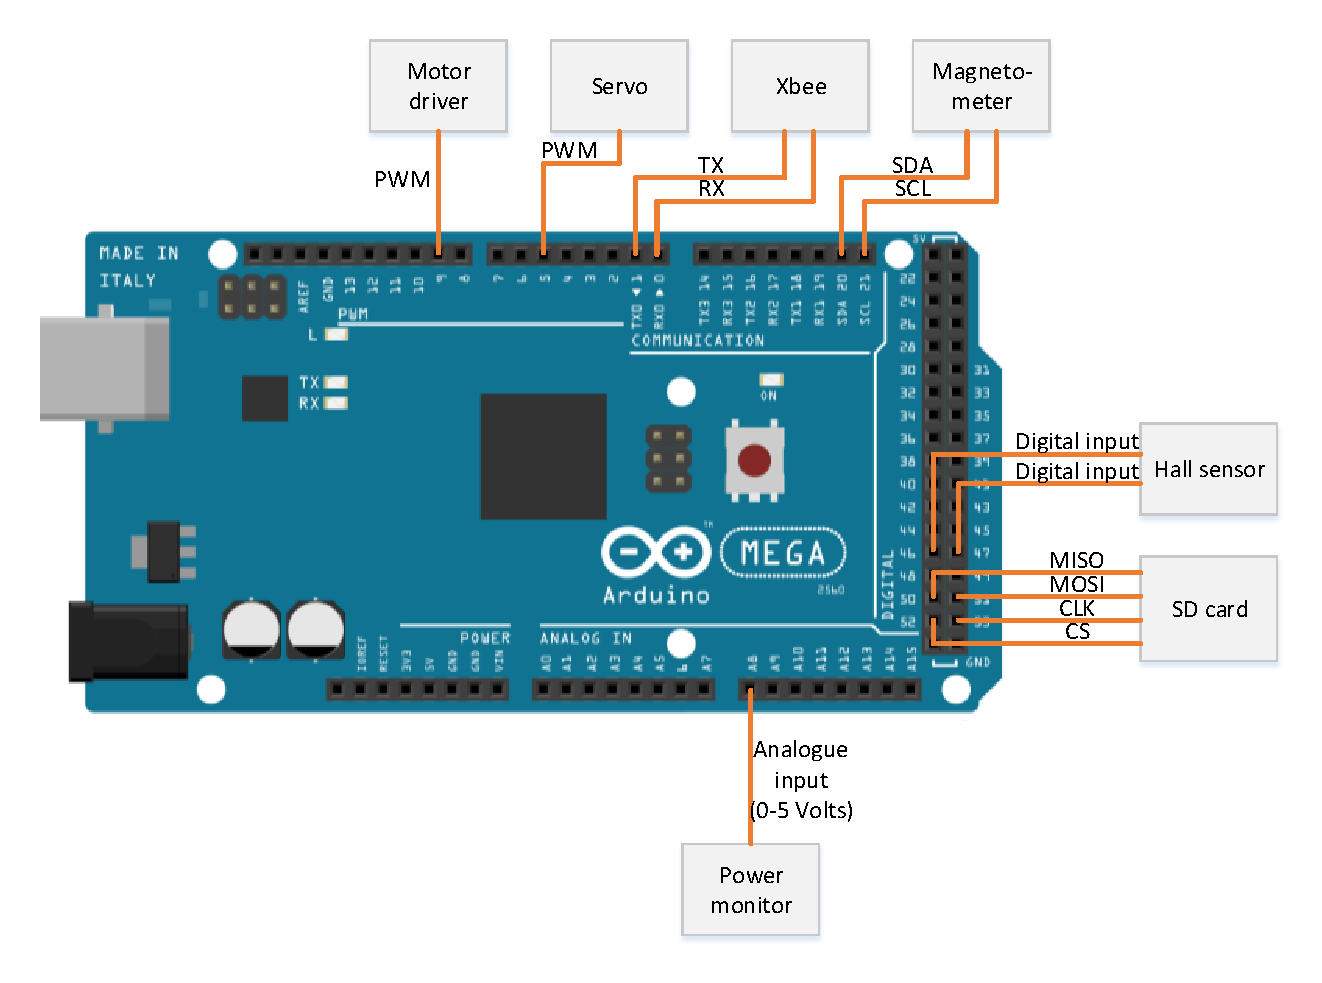
\includegraphics[scale=0.75]{figures/MegaSetup.pdf}
	\caption{Connections between the different hardware components and the Arduino.}
	\label{MegaSetup}
\end{figure}

The XBee module needs to connect to a serial port, and UART3 is chosen, as it makes it easier to route the PCB traces. UART3 is located at pins 0 and 1. 

The SD card needs an SPI connection, and must therefore be connected to the SPI pins 50, 51, 52 and 53. 

The "9 Degrees of Freedom" board needs an $\text{I}^2\text{C}$ connection, and has to be connected to the Arduino's $\text{I}^2\text{C}$ pins 20 and 21. 

The PWM signals sent to the motor and servo can be set to any of the PWM pins. For easier routing, pin 9 for the motor and pin 5 for the servo is selected.

The input from the hall sensors will be measured by the input capture pins (ICP4 and ICP5), to which Timer 4 and Timer 5 are connected. On the Arduino board, it corresponds to the pins 46 and 47.

Lastly, the voltage divider used for the power monitoring is connected to an analogue pin chosen to be pin A9.

As all hardware modules have now been assigned pins on the Arduino, the electrical requirements of each module will now be considered.

\subsection{Electrical considerations}\label{sec:elecConsiderations}

Before connecting hardware modules to the Arduino pins, signal voltage levels also need to be considered:

\begin{itemize}
\item The Arduino Mega 2560 itself uses 5V logic levels.\cite{MegaInfo}
\item The "9 Degrees of Freedom" board needs \SI{3,3}{V}-\SI{16}{V} supply and $\SI{3,3}{V}$ logic levels. \cite{9dog}
\item The servo needs $\SI{4,8}{V}$ to \si{6\ V} supply voltage and signal levels.\cite{futaba}
\item The SD card needs $\SI{3,3}{V}$ supply voltage and signal levels, see \subsecref{SDcard}.
\item The Hall sensors needs $\SI{3,5}{V}$ to \si{24\ V} supply, and a pull up resistor to define the logic level.
\cite{HallDS}
\item The XBee module needs $\SI{3,3}{V}$ supply voltage and signal levels.
\subsecref{Xbee}
\end{itemize} 

The Arduino has regulated 5V and $\SI{3,3}{V}$ supply rails available, which will be used to power the respectable hardware modules. As the servo can potentially draw a lot of current, and overload the Arduino, it will be connected to a dedicated 5V voltage regulator, powered directly from the battery.

A low-dropout type is chosen, L4941, to make sure it works, even at low battery voltages. This regulator has a maximum dropout of 700mV at 1A current, meaning that it will work with battery voltages as low as $\SI{5,7}{V}$. \cite{L4941} 

All one-directional connections from the Arduino to  $\SI{3,3}{V}$ logic level inputs will be connected to a HEF4050 CMOS buffer. This device can accept input voltages up to 15V, while supplied by as little as 3V supply voltage \cite{4050B}. This makes it ideal for uni-directional voltage level translation. 

One-directional connections from  $\SI{3,3}{V}$ logic level output to Arduino inputs will be connected directly, as $\SI{3,3}{V}$ is above the minimum high level threshold \cite{Atmega}.
%
\begin{flalign}
\eq{V_{IH,min}}{0,6 \cdot V_{cc}}& \nonumber \\
\eq{V_{IH,min}}{0,6 \cdot 5}& \nonumber \\
\eq{V_{IH,min}}{3} \si{\ V}& \nonumber
\end{flalign}

As the $\text{I}^2\text{C}$ bus is using bi-directional connections, and needs to connect a $\SI{3,3}{V}$ system to a 5V system, this needs to be addressed as well. One solution could be running the bus at $\SI{3,3}{V}$, but this is unfortunately not possible, as the microcontroller needs at least $\SI{3,5}{V}$ as HIGH voltage, when in  $\text{I}^2\text{C}$ mode \cite{Atmega}. The creators of $\text{I}^2\text{C}$, Philips, recommend solving this with two MOSFETs, see \figref{i2clevel}.

\begin{figure}[H]
	\centering
	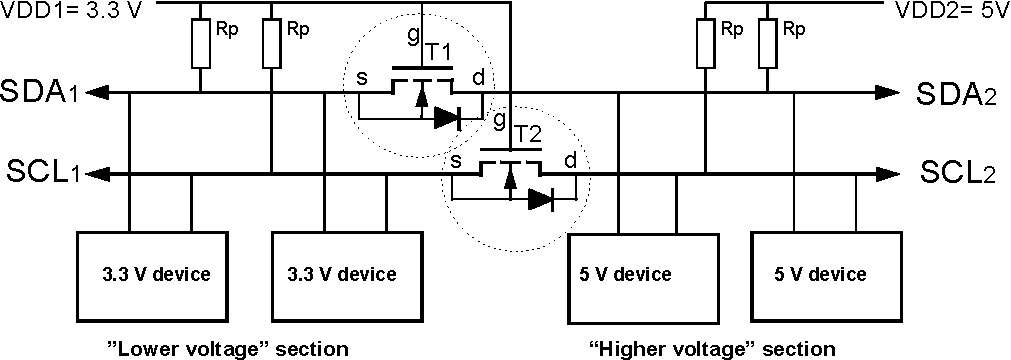
\includegraphics[scale=0.9]{figures/i2cLevel.pdf}
	\caption{$\text{I}^2\text{C}$ Voltage level translator. [source: Philips]}
	\label{i2clevel}
\end{figure}

\todo{Source to picture Thomas}

In $\text{I}^2\text{C}$ systems, the nodes can only pull the line LOW. To make it possible to signal a HIGH, pull-up resistors are used. If a low voltage system is directly connected to a higher voltage system, the voltage at the input pins of the low-voltage section risk being pulled up to 5V.

To solve this, the translator uses a MOSFET per signal line, with the gate connected to the lower supply voltage, to separate the two systems. Here is a quick explanation, examining just one line (as both lines are implemented identically):\\
%
The gate of the MOSFET is connected to \SI{3,3}{V}.
Four states are possible, both sides HIGH, both sides LOW, or one of each.
If both ends are in the HIGH state, the voltage on the source pin will be \SI{3,3}{V}, and the gate-source voltage will therefore be $\SI{3,3}{V}-\SI{3,3}{V}=\SI{0}{V}$. The MOSFET is therefore off, and not conducting. This prevents the 5V supply from reaching the input of the \SI{3,3}{V} side.\\
If the \SI{3,3}{V} section is in the LOW state, the voltage on the source pin will be 0V, and the gate-source voltage will therefore be $\SI{3,3}{V}-\SI{0}{V}=\SI{3,3}{V}$, turning the MOSFET on. This in turn pulls the 5V section to 0V, signalling a LOW.\\
If the 5V voltage section is in the LOW state, the intrinsic diode in the MOSFET will conduct, pulling the source pin down to \si{0\ V} plus a diode drop ($\approx\SI{0,6}{V}$). This results in a gate-source voltage of $\SI{3,3}{V}-\SI{0,6}{V}=\SI{2,7}{V}$, turning the MOSFET on. This will eliminate the diode drop, and the result will be 0V on the source pin, signalling a LOW to the \SI{3,3}{V} side.

For this to work, a MOSFET that will turn on at \SI{2,7}{V} is needed. FDV303N is available and choosen, as it has a $\text{V}_\text{ds}$ threshold voltage\footnote{The  $\text{V}_\text{ds}$ threshold is the voltage, where the MOSFET starts to conduct} of maximum \SI{1,5}{V}. At \SI{2,7}{V}, the drain-source resistance is specified to \SI{0,6}{\Omega}, meaning that the MOSFET will be on at this voltage\cite{MOSFET}.

\subsection{Voltage divider}

The power monitor need a voltage divider, see \secref{Hardwarechoice}. With a measurement interval of 0 to 5 volts in 1023 steps for the analogue pin on the Arduino, the voltage divider has to be designed to be able measure the whole interval for the battery pack. As the battery pack can have a voltage up to \si{9,0\ V}\cite{BatteryDS}, the transfer constant for the voltage divider need to be smaller than 0,59 to measure the whole interval. The smaller the transfer constant, the bigger the interval is and the bigger each step will be. To make sure that there will not come a bigger voltage than 5 volts on the output from the voltage divider, the transfer constant is set to 0,5: this will give a maximum voltage into the voltage divider of 10 volts before the output voltage goes beyond 5 volts. To get a transfer constant of 0,5, the resistors in the voltage divider have to be the same, see \eqref{VolDivRes3}.\\
%
If,
\begin{flalign}
R &= R_1 = R_2  \unit{\Omega} \nonumber\\
\text{Then,}\nonumber\\
\eq{V_{out}}{\frac{R}{R + R} \cdot V_{in}}\unit{V} \nonumber \\
\eq{V_{out}}{\frac{1}{2} \cdot V_{in}}\unit{V}
\label{VolDivRes3}
\end{flalign}
%
For the size of the resistors, the output impedance for the voltage divider have to be taken into consideration. For the analogue pins on the Arduino, it is recommended to have a output impedance smaller than \si{10\ k\Omega}, or the it will begin to disturb the reading on the pin.\\
To make sure that this does not happen, the resistors in the voltage divider are set to half of the maximum output impedance, \si{5\ k\Omega}. The closest resistor in the E96 series is \si{4,99\ k\Omega}, which will be used for both resistors. 

The final voltage divider circuit for the power monitor can be seen on \figref{VoltDivFigFinal}.
\begin{figure}[h!]
\centering
\begin{circuitikz}
\draw (0,2)
to[short,l=$V_{in}$] (1,2)
to[short] (2,2)
to[R=$R_1$] (2,0)
to[R=$R_2$] (2,-2);
\draw (2,-2) 
to[short] node[ground] {} (2,-3);
\draw (2,0)
to[short] (3,0)
to[short,l=$V_{out}$] (4,0);
\draw (2,0)
to[C=$C_1$] (0,0)
to[short] node[ground] {} (0,-1);
\end{circuitikz}
\caption{The implemented voltage divider} 
\label{VoltDivFigFinal}
\end{figure}

To filter the high frequency noise out, a simple low-pass RC filter is finally implemented with a 1 $\mu$F capacitor in the voltage divider. The resulting cut-off frequency is then:
%
\begin{flalign}
\eq{\omega_{c}}{\frac{1}{R \cdot C}}\unit{rad \cdot s^{-1}} \nonumber \\
\eq{\omega_c}{\frac{1}{2,5 \cdot 10^{3} \cdot 1 \cdot 10^{-6}}}\unit{rad \cdot s^{-1}} \nonumber \\
\eq{\omega_c}{400}\si{\ rad \cdot s^{-1}}&\nonumber
\end{flalign}

With all the hardware components physically implemented on the vehicle and connected to the microcontroller, the software utilized needs to be determined and designed to enable interactions between the Arduino and all the hardware components.